%----------------------------------------------------------------------------------------
%   PACKAGES & CONFIGURATIONS DU DOCUMENT
%----------------------------------------------------------------------------------------

\documentclass[12pt]{article}
\usepackage[english]{babel}
\usepackage[utf8x]{inputenc}
\usepackage{amsmath}
\usepackage{graphicx}
\usepackage{float}
\usepackage[toc,page]{appendix}
\renewcommand\appendixpagename{Annexe}
\renewcommand\appendixtocname{Annexe}
\usepackage[textwidth=17cm,textheight=22cm]{geometry}
\usepackage[colorinlistoftodos]{todonotes}

\begin{document}

\begin{titlepage}

\newcommand{\HRule}{\rule{\linewidth}{0.2mm}} % Commande définie pour les lignes horizontales (changer l'épaisseur ici)

\center % Centre tout sur la page
 
%----------------------------------------------------------------------------------------
%   TITRES
%----------------------------------------------------------------------------------------

\textsc{\LARGE Documentation}\\[3.0cm] % Nom de l'université

%----------------------------------------------------------------------------------------
%   LOGO
%----------------------------------------------------------------------------------------


\includegraphics[scale=1]{logoSEO.png}\\[3.0cm] % Logo de l'entreprise

%----------------------------------------------------------------------------------------
%   TITRE PRINCIPAL
%----------------------------------------------------------------------------------------

\HRule \\[0.5cm]
{ \huge \bfseries SEO Echo}\\[0.2cm] % Titre du document
\HRule \\[1.5cm]

%----------------------------------------------------------------------------------------
%   AUTEUR
%----------------------------------------------------------------------------------------

\centering \large
Julien \textsc{Cordat-Auclair}\\[1cm] % Nom

%----------------------------------------------------------------------------------------
%   DATE
%----------------------------------------------------------------------------------------

{\large 13 août 2018}\\[3cm] % Date

%----------------------------------------------------------------------------------------
%   LOGO
%----------------------------------------------------------------------------------------


\includegraphics[scale=1]{logocometnet.png}\\[1cm] % Logo de l'entreprise
 
%----------------------------------------------------------------------------------------

\vfill % Remplir le reste de la page avec des lignes vides

\end{titlepage}

%----------------------------------------------------------------------------------------
%   PLAN
%----------------------------------------------------------------------------------------

\renewcommand{\contentsname}{Table des matières}

\tableofcontents{}

%----------------------------------------------------------------------------------------
%   RAPPORT
%----------------------------------------------------------------------------------------

%----------------------------------------------------------------------------------------
%   PRESENTATION GENERALE
%----------------------------------------------------------------------------------------

\newpage
\section{Présentation générale}

\texttt{SEO Echo} est un service permettant de soumettre des recommandations à un utilisateur vis-à-vis du contenu de sa page web pour qu'il puisse optimiser le référencement de celle-ci en fonction d'une requête donnée. Il y a donc 2 paramètres que l'utilisateur doit fournir : l'URL de sa page et des mots-clés qui constituent la requête pour laquelle l'utilisateur souhaite voir sa page mieux placée dans les résultats de recherche Google.

\

Afin de mettre en place ce projet, l'idée est d'utiliser l'algorithme d'apprentissage machine \texttt{Echo} de manière à extraire les termes qui permettent de différencier un site bien référencé d'un site mal référencé pour une requête donnée. Ce sont ces termes qui seront proposés à l'utilisateur. 3 étapes distinctes apparaissent alors :
\begin{itemize}
	\item \underline{1ère étape :} le web scraping. Lors de cette étape, on récupère des données afin de pouvoir faire fonctionner l'algorithme \texttt{Echo}. Ces données correspondent au contenu présent dans les balises HTML (que l'on choisit) des \textit{n} pages web les mieux référencées pour la requête donnée, l'entier \textit{n} pouvant être modifié.
	
	\item \underline{2ème étape :} l'apprentissage machine. On fournit les données précédemment récupérées à \texttt{Echo} qui retourne les termes qui permettent d'être mieux référencé (via \texttt{EchoBT}) mais aussi une estimation de la position de la page de l'utilisateur (via \texttt{EchoPos}) et un taux de performance permettant de rendre compte de la pertinence des résultats de chacun des deux algorithmes précédents (via \texttt{EchoV}).
	
	\item \underline{3ème étape :} l'UX design. C'est l'optimisation de l'affichage des résultats renvoyés par \texttt{Echo} à partir des données fournies.
\end{itemize}
	
\

Avant de détailler chacune des étapes présentées ci-dessus, voici un exemple concret de l'action de SEO Echo. Le premier tableau représente les données fournies par l'utilisateur et le second correspond aux résultats renvoyés par \texttt{Echo} :

\

\

\begin{center}
\begin{tabular}{|c|c|}
\hline
URL de l'utilisateur & http://com-et-net.com \\
\hline
Mots-clés & stratégie digitale grenoble \\
\hline
\end{tabular}

\

\

\begin{tabular}{|c|c|c|}
\hline
\texttt{EchoBT} & référencement\_title, agence\_title, stratégie\_alt, isère\_strong ... \\
\hline
\texttt{EchoPos} & 14 \\
\hline
\texttt{EchoV} & 0.76, 0.63 \\
\hline
\end{tabular}
\end{center}

%----------------------------------------------------------------------------------------
%   PREMIERE PARTIE
%----------------------------------------------------------------------------------------

\newpage
\section{Le web scraping}

\textit{pour plus d'information, se référer aux commentaires dans le code}

\

\

Voici un schéma représentant l'architecture de cette première étape :

\

\begin{center}
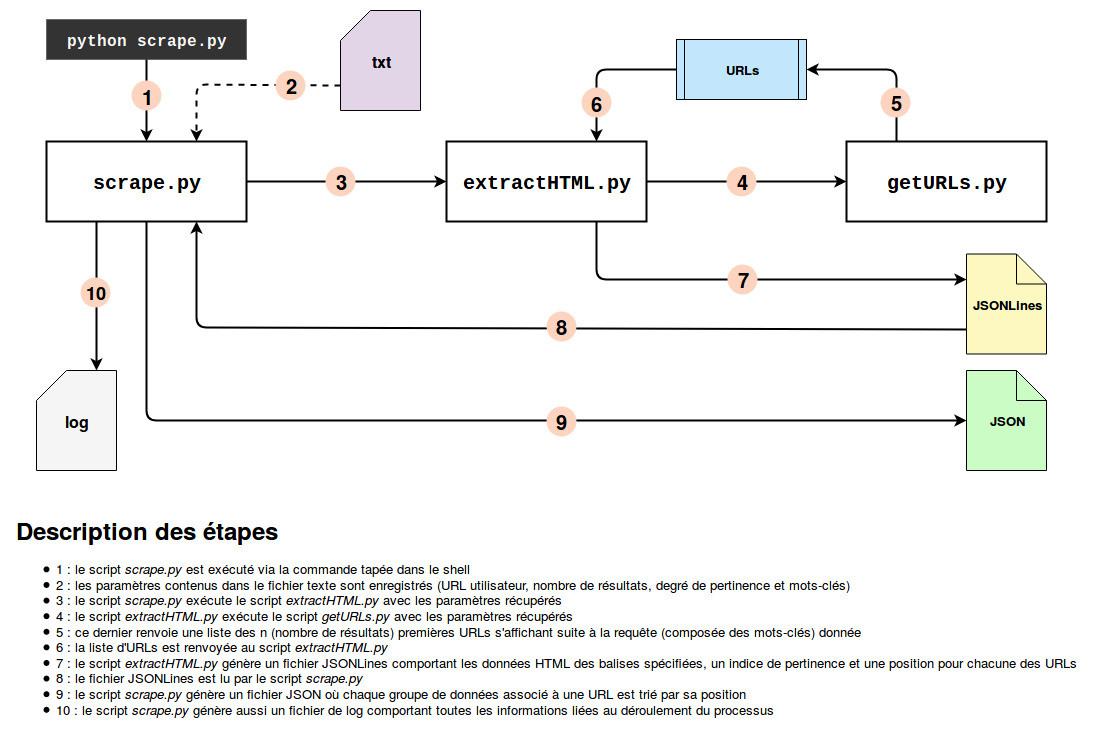
\includegraphics[scale=0.45]{architectureScraping.jpg}
\end{center}

\newpage
\underline{\texttt{scrape.py} :} c'est le script principal qui permet de lancer le processus de web scraping.
\begin{itemize}
 	\item \textbf{log} : le script génère un fichier de log qui permet de suivre le déroulement du processus et ainsi de repérer les éventuelles erreurs pouvant survenir. Il est écrasé à chaque exécution et se trouve dans le dossier \textit{/CrawlGooglePython/bin/log}.
 	
 	\item \textbf{paramètres} : le script est également en mesure de lire un fichier texte en interprétant son contenu de la manière suivante :
 	
 	\begin{center}
	 \begin{tabular}{|c|c|c|c|}
	\hline
	1ère ligne  & URL de l'utilisateur \\
	\hline
	2ème ligne & nombre de pages à étudier \\
	\hline
	3ème ligne & degré de pertinence \\
	\hline
	lignes suivantes & mots-clés \\
	\hline
	\end{tabular}
	\end{center}
	
	\item \textbf{lancement du processus} : les paramètres précédemment récupérés sont utilisés pour appeler le script \texttt{extractHTML.py} qui permet d'initialiser le web crawling (voir plus loin).
	
	\item \textbf{tri des résultats} : une fois les résultats du web crawling obtenus, le script est capable de trier le fichier \texttt{JSONLines} que \texttt{Scrapy} génère et contenant les données \texttt{HTML} (désordonnées car \texttt{Scrapy} est asynchrone) en fonction de la position de chacune des pages étudiées. 
	
	\item \textbf{génération d'un fichier de sortie} : un nouveau fichier \texttt{JSON} (et non \texttt{JSONLines}) est créé de manière à ce qu'il puisse être lu plus tard par le script \texttt{PHP} (\texttt{PHP} ne lit pas les fichiers \texttt{JSONLines}). Il se trouve dans le dossier \textit{/CrawlGooglePython/bin/searchEngine/output} et se nomme \textit{output.json}.
\end{itemize}

\newpage
\underline{\texttt{extractHTML.py} :} c'est le script capable d'extraire les données \texttt{HTML} des pages web. Il utilise le framework \texttt{Scrapy}.
\begin{itemize}
	\item \textbf{cleanHTML} : fonction chargée de nettoyer le contenu extrait des pages web car \texttt{Echo} n'est pas capable de traiter les données avec des accents, des signes de ponctuation ou encore des espaces vides.
	\item \textbf{cleanURL} : fonction chargée de nettoyer une URL. Elle est utilisée lorsque l'on souhaite récupérer les mots-clés présents dans le lien de la page et séparés par des anti-slashs.
	\item \textbf{lancement de la récupération d'URLs} : afin de collecter les données des pages web, encore faut-il avoir ces pages à disposition. C'est pourquoi le script permet d'exécuter \texttt{getURLs.py} (voir plus loin) grâce aux paramètres précédemment transmis par \texttt{scrape.py}.
	\item \textbf{start\_requests} : fonction chargée d'attribuer à chaque URL récupérée sa position dans la page de recherche Google ainsi qu'un indice de pertinence. Par exemple, si le degré de pertinence vaut 30, alors les 30 premières pages auront un indice de pertinence de 1 et les autres de 2. On attribue par ailleurs à la page de l'utilisateur (elle aussi étudiée) la position 0 et un indice de pertinence de 0.
	\item \textbf{parse} : fonction principale de ce script chargée de récupérer le contenu des balises spécifiées pour les URLs récupérées. Cette fonction génère un fichier \texttt{JSONLines} se trouvant dans le dossier \textit{/CrawlGooglePython/bin/searchEngine/output} et se nommant \textit{unsortedOutput.jsonl}. Si l'on souhaite modifier les balises à étudier, il faut penser à modifier le fichier \textit{/CrawlGooglePython/bin/searchEngine/items.py}. 
\end{itemize}

\newpage
\underline{\texttt{getURLs.py} :} c'est le script permettant de récupérer les \textit{n} premières URLs affichées pour une requête donnée, il utilise le framework \texttt{Selenium}.
\begin{itemize}
	\item \textbf{génération d'une fenêtre Firefox} :  \texttt{Selenium} permet de simuler une requête Google en générant une fenêtre d'un navigateur donnée. Ici, on utilise Firefox.
	\item \textbf{génération de la requête} : une fois le navigateur lancé, la requête est créée à partir des mots-clés de l'utilisateur puis transformée en une URL. Ce lien spécifie également le nombre de résultats à afficher : si \textit{n} est inférieur à 100 (limite imposée par Google quant au nombre de résultats à afficher sur une seule page de recherche), alors exactement \textit{n} résultats seront présents sur la page générée. Sinon, une première page avec 100 résultats sera créée puis une seconde avec le nombre de résultats restants sera générée plus tard. La limite est donc de 200 résultats, mais on peut l'étendre en répétant simplement cette méthode.
	\item \textbf{récupération des URLs} : une fois la page de recherche générée, le script permet de récupérer les URLs de chacun des liens présents en identifiant les balises qui identifient leur présence. Ces liens sont ensuite stockés dans une liste qui est renvoyée à la fin du processus.
	\item \textbf{gestion d'erreur} : entre temps, plusieurs erreurs sont gérées. On vérifie que la page n'est pas vide, que Google n'a pas supprimé de lien pour des droits d'auteurs ou encore qu'un lien vers Google image n'est pas présent. Dans le premier cas, le processus est arrêté. Pour les autres, un message d'information est affiché. Enfin, Google peut décider d'afficher un code captcha qui empêche la récupération des URLs et le script est capable de le repérer pour pouvoir informer l'utilisateur de ce problème.
\end{itemize}

%----------------------------------------------------------------------------------------
%   DEUXIEME PARTIE
%----------------------------------------------------------------------------------------

\newpage
\section{L'apprentissage machine}

\textit{pour plus d'information, se référer aux commentaires dans le code}

\

\

Voici un schéma représentant l'architecture de cette première étape :

\

\begin{center}
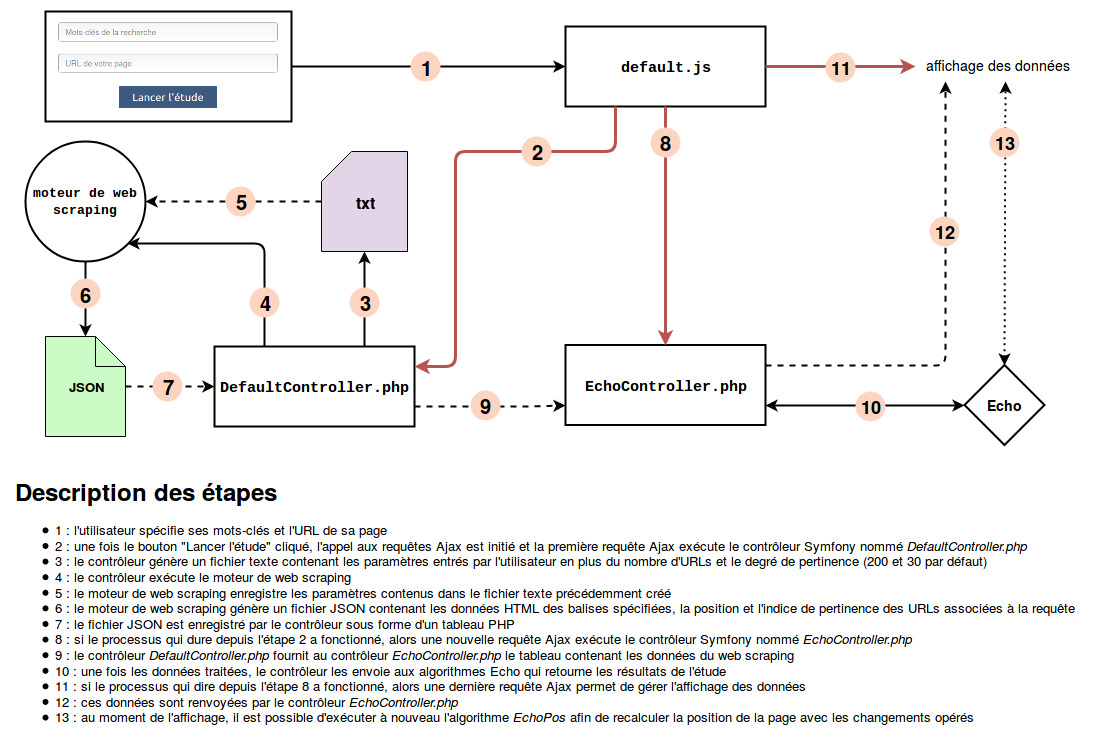
\includegraphics[scale=0.45]{architectureMachineLearning.jpg}
\end{center}

\newpage
\underline{\texttt{default.js} :} c'est le script qui fait le lien entre l'affichage des résultats et le calcul de ces derniers. Il va notamment permettre d'appeler les scripts \texttt{PHP} les uns après les autres une fois que l'utilisateur aura décidé de lancer l'étude grâce à des requêtes \texttt{Ajax} imbriquées. Cela permet à la fois d'optimiser la gestion d'erreur (puisqu'il est facile de savoir lors de quelle étape le processus a rencontré une erreur) mais aussi l'affichage (car les pages sont générées rapidement).

\newpage
\underline{\texttt{defaultController.php} :} c'est le premier script exécuté une fois le bouton de lancement cliqué. C'est aussi celui qui fait le lien entre l'étape de web scraping et celle de machine learning.
\begin{itemize}
	\item \textbf{écriture du fichier de paramétrage} : le script permet de récupérer les données entrées par l'utilisateur avant de lancer le processus, soit son URL et ses mots-clés. Ces paramètres sont ensuite écrits dans le fichier texte que \texttt{scrape.py} va pouvoir lire plus tard. Ils sont accompagnés du nombre de résultats à étudier (\textit{nResults}) et du degré de pertinence (\textit{efficiency}). Ces valeurs sont codées dans le dur et peuvent être modifiées à tout moment.
	\item \textbf{lancement du web scraping} : une fois le fichier de paramétrage créé, le processus de web scraping présenté précédemment est lancé et les résultats sont récupérés depuis le fichier de sortie \textit{output.json}.
	
\newpage
\underline{\texttt{echoController.php} :} c'est le script qui permet de formater les données puis de les envoyer à \texttt{Echo}.
	\item \textbf{conversion du fichier de sortie} : le fichier \texttt{JSON} (\textit{output.json}) est récupéré puis transformé en un tableau \texttt{PHP} afin de pouvoir modifier les données qu'il contient. En réalité, il est même séparé en deux tableaux ; l'un contient les données de tous les résultats issus de la recherche Google (\textit{arrayGoogleResults}), l'autre contient les données de la page de l'utilisateur (\textit{arrayUserSite}).
	
	\item \textbf{récupération des meilleures pages} : le script est capable de récupérer les 10 pages les mieux référencées pour la requête donnée afin de pouvoir les afficher plus tard.
	
	\item \textbf{formatage des données} : le script permet de faire le lien avec \texttt{Echo}, mais ce dernier ne peut pas lire les données telles quelles. Un nouveau tableau (\textit{tabResGoogle}) et donc créé afin d'y stocker les données modifiées de manière à ce que \texttt{Echo} puisse les lire. Ainsi, le tableau contient 4 champs pour chaque page : un identifiant (l'URL), une position, un degré de pertinence et une chaîne de prédicteurs. Cette chaîne est en fait composée de tous les termes confondus et avec comme suffixe le nom de la balise qui leur est associée individuellement (par exemple, \textit{agence\_TITLE}). Le même traitement est opéré pour la page de l'utilisateur.
	
	\item \textbf{duplication des pages pertinentes} : \texttt{Echo} se sert de la notion de pertinence pour pouvoir identifier les termes qui sont importants vis-à-vis du référencement. Un terme qui apparaît sur des pages pertinentes et non pertinentes n'est pas un terme important, mais un terme qui apparaît sur des pages pertinentes et non sur les pages non pertinentes l'est. Afin d'amplifier ce mécanisme, les pages pertinentes sont dupliquées de la manière suivante dans le code : 
	\begin{itemize}
		\item les pages allant de la position 1 à \textit{n1} sont multipliées \textit{coeff1} fois
		\item les pages allant de la position \textit{n1} à \textit{n2} sont multipliées \textit{coeff2} fois
		\item les pages allant de la position \textit{n2} à \textit{n3} sont multipliées \textit{coeff3} fois
	\end{itemize}
Toutes ces valeurs sont évidemment modifiables.

	\item \textbf{appel aux algorithmes} : une fois les données traitées, les algorithmes \texttt{EchoBT}, \texttt{EchoPos} et \texttt{EchoV} peuvent être appelés. En ce qui concerne \texttt{EchoBT}, il est possible de modifier le nombre de termes à renvoyer dans le fichier \textit{echobt/Network.java} via la constante \textit{nb}.
	
	\item \textbf{triPredicteurs} : les meilleurs termes renvoyés peuvent avoir des formes très variables. Dans certains cas par exemple, énormément de mots de la balise \textit{alt} sont proposés. Ainsi, cette fonction permet de spécifier le nombre de termes à renvoyer par balise. Ces valeurs peuvent être modifiées librement à travers les constantes \textit{nbTitle}, \textit{nbUrl}, \textit{nbH1}, ... De plus, cette fonction permet de renvoyer les résultats triése par ordre d'importance de balise (et par score au sein de chaque balise).
	
	\item \textbf{refreshAction} : cette fonction permet de recalculer la position de la page après que l'utilisateur ait modifié son contenu (voir plus loin). Le nouvel objet \texttt{JSON} contenant les nouvelles données est récupéré via une variable \texttt{POST}, puis le traitement des données est effectué pour ensuite appeler \texttt{EchoPos} et renvoyer le résultat.
\end{itemize}

%----------------------------------------------------------------------------------------
%   TROISIEME PARTIE
%----------------------------------------------------------------------------------------

\newpage
\section{L'UX design}

\

\textit{pour plus d'information, se référer aux commentaires dans le code}

\

\

Voici des captures de l'affichage des résultats :

\begin{center}
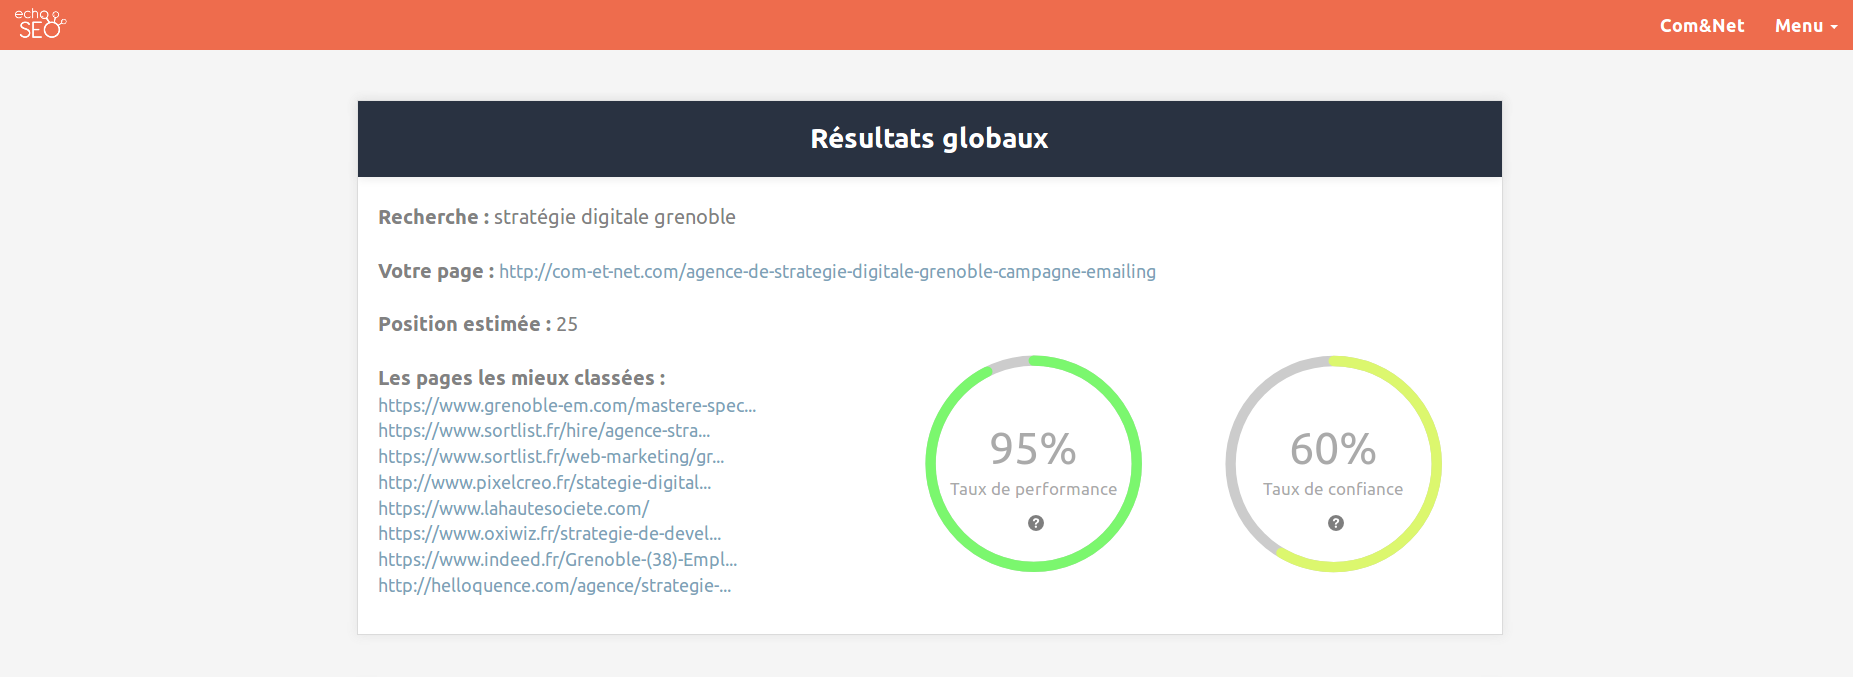
\includegraphics[scale=0.25]{hautDePage.png}

\

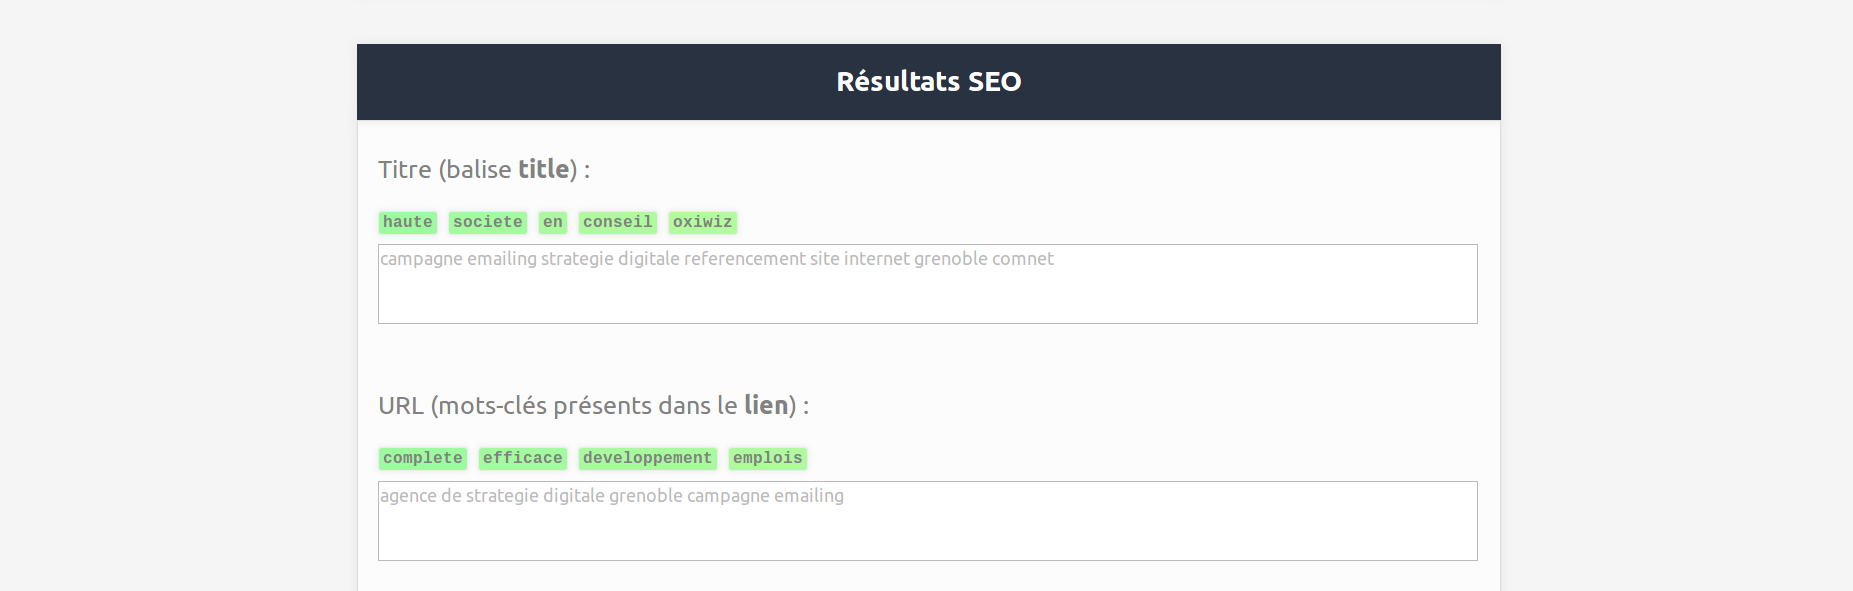
\includegraphics[scale=0.25]{milieuDePage.png}

\

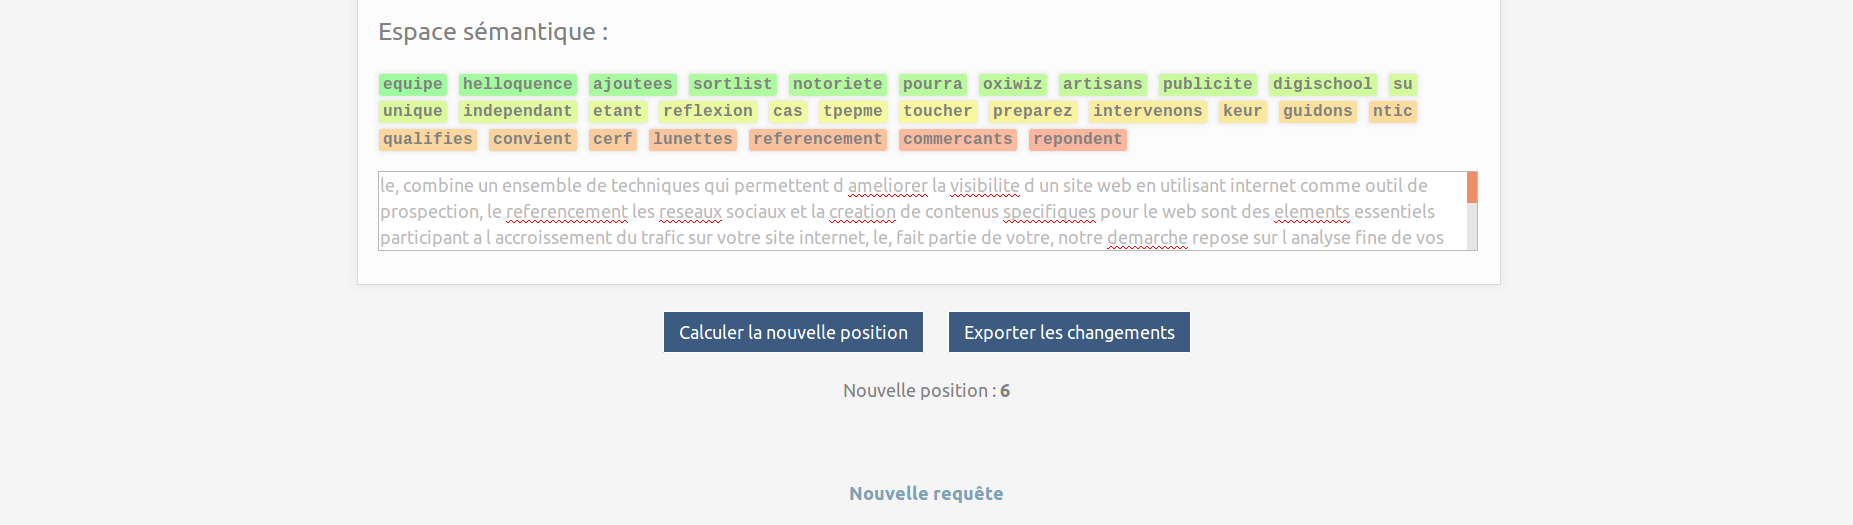
\includegraphics[scale=0.25]{basDePage.png}

\

\end{center}

\newpage
Pour cette étape, la majorité du travail se trouve dans le fichier \textbf{default.js} situé dans le dossier \textit{/echoSEOBundle/Resources/public/js} (même si les fichiers \texttt{HTML} et \texttt{CSS} permettent d'y participer grandement). Une fois que toutes les requêtes \texttt{Ajax} se sont déroulées sans qu'aucune erreur ne se produise, la page de résultat est générée. Elle se divise en deux sections distinctes : la première comporte des informations générales vis-à-vis de l'étude menée, la seconde présente les meilleurs termes qui en ressortent.

\

Au niveau de la première section, deux graphes correspondant aux résultats renvoyés par \texttt{EchoV} sont générés. Leur couleur varie en fonction de la valeur du pourcentage qui leur est associé. Les 10 meilleures URLs sont également affichées ainsi que la position estimée de la page (\texttt{via EchoPos}) et les données entrées par l'utilisateur.

\

Quant à la seconde section, elle comporte les termes renvoyés par \texttt{EchoBT} triés par ordre d'importance de balise et par score au sein de celles-ci. Une couleur est aussi associée à ces termes et permet de rendre compte de l'importance de ces derniers. Chacune des sous-sections formées par les balises comporte un champ de texte dans lequel est écrit le contenu dans la balise correspondante de la page de l'utilisateur. Ce texte peut être modifié en se basant notamment sur les termes proposés. Une fois les changements opérés, l'utilisateur peut cliquer sur le bouton intitulé ''Calculer la nouvelle position'' afin d'estimer la position de la page si les modifications avaient vraiment eu lieues. Enfin, si l'utilisateur le souhaite, il peut les exporter via le bouton correspondant : un fichier \texttt{JSON} est alors proposé au téléchargement et il contient toutes les données inscrites dans les champs de texte (modifiés ou non). Il lui suffira ensuite de copier/coller ce contenu dans les balises associées (dans son code) pour pouvoir réellement améliorer le référencement de sa page web.

\end{document}